%%%%%%%%%%%%%%%%%%%%%%% file template.tex %%%%%%%%%%%%%%%%%%%%%%%%%
%
% This is a template file for Web of Conferences Journal
%
% Copy it to a new file with a new name and use it as the basis
% for your article
%
%%%%%%%%%%%%%%%%%%%%%%%%%% EDP Science %%%%%%%%%%%%%%%%%%%%%%%%%%%%
%
%%%\documentclass[option]{webofc}
%%% "twocolumn" for typesetting an article in two columns format (default one column)
%
\documentclass{webofc}
\usepackage[varg]{txfonts}   % Web of Conferences font
%
% Put here some packages required or/and some personnal commands
%
%
\begin{document}
%
\title{Evolution of the CMS Submission Infrastructure to Support Heterogeneous Resources}
%
% subtitle is optionnal
%
%%%\subtitle{Do you have a subtitle?\\ If so, write it here}

\author{
        \firstname{M.} \lastname{Mascheroni}\inst{1} \fnsep\thanks{\email{marco.mascheroni@cern.ch}} \and
        \firstname{A.} \lastname{P\'erez-Calero Yzquierdo}\inst{2,3} \and
        \firstname{M.} \lastname{Acosta Flechas}\inst{4} \and
        \firstname{J.} \lastname{Dost}\inst{1} \and
        \firstname{S.} \lastname{Haleem}\inst{5} \and
        \firstname{K.} \lastname{Hurtado Anampa}\inst{6} \and
        \firstname{F. A.} \lastname{Khan}\inst{4} \and
        \firstname{E.} \lastname{Kizinevi\v{c}}\inst{7} \and
        \firstname{N.} \lastname{Peregonov}\inst{4}, for the CMS Collaboration.
}

\institute{
    University of California San Diego, La Jolla, CA, USA\and
    Centro de Investigaciones Energ\'eticas, Medioambientales y Tecnol\'ogicas (CIEMAT), Madrid, Spain \and
    Port d'Informaci\'o Cientifica (PIC), Barcelona, Spain \and
    Fermi National Accelerator Laboratory, Batavia, IL, USA \and
    National Centre for Physics, Islamabad, Pakistan \and
    University of Notre Dame, Notre Dame, IN, USA \and
    European Organization for Nuclear Research, Meyrin, Switzerland
}

\abstract{%
The landscape of computing power available for the CMS experiment is expected to evolve in the future from almost exclusively x86 processors predominantly deployed at WLCG sites towards a more diverse mixture of Grid, HPC, and Cloud facilities incorporating a higher fraction of non-CPU components such as GPUs. Using these facilities' heterogeneous resources efficiently to process the vast amounts of data to be collected in the HL-LHC era is key to CMS's achieving its scientific goals. Workload management and resource provisioning tools will need to evolve, taking into account the optimal level of granularity in the description of the resources for efficient allocation and matchmaking to tasks. Open questions include what types of resources will be available in the future, how to prioritize diverse workflows to those diverse types, as well as the policy preferences of the resource providers themselves. The descriptions of the tasks and the properties of the resources, as well as CMS or local use policies including resource validation, i.e. suitability to run a particular workflow, must be taken into account. This contribution describes the present capabilities of the CMS Submission Infrastructure and its critical dependencies on the underlying tools (such as HTCondor and GlideinWMS), along with its necessary evolution towards a full integration and support of heterogeneous resources according to the CMS needs.
}
%
\maketitle
% ----------------

\section{Introduction}
\label{sec:intro}
The Submission Infrastructure (SI) Group of the CMS experiment at CERN manages the computing infrastructure dedicated to the processing, reconstruction, simulation, and analysis of physics data. The SI team makes use of GlideinWMS~\cite{gwms} and HTCondor~\cite{htcondor} software as basic tools to build and run a Global Pool~\cite{global_pool} of computing resources. Our activities include the ordinary operations of this infrastructure, while preparing for future scales and requirements, integrating new resource types to be employed by CMS, and acting as liaison with the HTCondor and GlideinWMS communities in order to stimulate and integrate new features, according to CMS priorities.  

This paper will summarize the readiness of the CMS SI to allocate, manage and provide heterogeneous (that is, not purely CPU) compute resources to support CMS data processing activities (section~\ref{sec:globalpool}). However, in order present the subject in the proper context, the motivation for the use of such heterogeneous resources (section~\ref{sec:motivation}), as well as the current (un)certainties in their utilization towards a CMS model (section~\ref{sec:model}), will be first briefly described. Finally, an updated perspective on the current status of the integration of heterogeneous resources into the CMS SI will be provided (section~\ref{sec:status}). 

% ========================================

\section{Motivation for the use of heterogeneous resources}
\label{sec:motivation}

The first incentive for the use of non-CPU resources is that they are expected to comprise an increasingly larger fraction of the computing power available to LHC experiments. In the current international landscape, with ever larger scientific projects and bigger scientific computing installations, growing funds are being committed to High Performance Computing (HPC) centers, looking onwards to reaching the Exascale. The LHC experiments, aware of such trends, are evolving their computing models towards the integration of these facilities~\cite{hpc}, which present the opportunity to help cover their growing computing demands. Additionally, CMS and the rest of collaborations are looking forward to gaining access to the best technologies available in the market, usually employed at the HPC facilities, many of which are built on heterogeneous architectures (e.g. CPU+GPU).

The LHC programme will enter in a High-Luminosity phase starting in 2027. The subsequent increase in data volumes will result in an unprecedented stream of scientific data, that will require vasts amounts of computing resources for its processing and analysis. The CMS collaboration has produced some estimates on its future computational needs~\cite{cms_hllhc}, and found that they will exceed in at least a factor four a simple extrapolation, by virtue of technology evolution, of the current capacities (see Fig.~\ref{cpu_cms2020}). In order to bridge the gap, a number of R\&D projects in CMS software are currently being developed~\cite{cms_RandD}, including the use of hardware accelerators, such as GPUs, to increase the data processing throughput with respect to CPUs for selected algorithms. The use of GPUs has been found to be particularly beneficial to event reconstruction tasks~\cite{gpus_track}.

\begin{figure}[h]
\centering
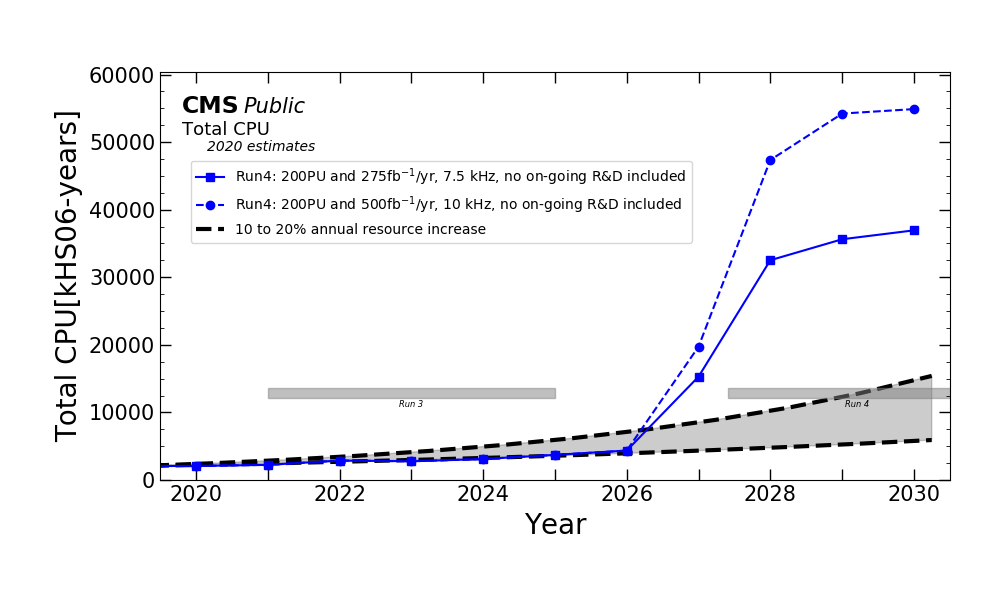
\includegraphics[width=11cm]{cpu_cms2020}
\caption{CMS computing resource needs projected into the HL-LHC era.}
\label{cpu_cms2020}
\end{figure}

The second motivational element can be thus found in the advantage that GPUs provide for certain data-intensive tasks. As an example, CMS has decided to adopt a heterogeneous solution for the High Level Trigger farm for the LHC Run 3~\cite{gpus_hlt}. CMS is interested in employing heterogeneous resources in HPC and Cloud clusters for offline computing as well. 

% ========================================

\section{Towards a model for CMS offline computing including GPUs}
\label{sec:model}

Considering the advantages of utilizing non-CPU resources, the LHC collaborations are currently undergoing a revision of their computing models, in order to incorporate them into their data processing and analysis plans. Making good use of the computing power available in heterogeneous infrastructures requires adapting not only the software layer, but also the workload management and resource provisioning systems, which are primarily designed for Grid CPU resources.

In the CMS case, The SI team must explore the use of new features in both GlideinWMS and HTCondor, in order to successfully allocate and manage heterogeneous resources. A set of tags to completely characterize these new slot types is required to ensure their most efficient matchmaking to CMS workloads. However, a number of uncertainties remain to this date. Therefore, beyond some current implementation examples, it is clear that the final model will likely be the result of an iterative process in which the unknowns described in this section are to be clarified.

First of all, accessing remote heterogeneous resources requires to take into consideration how they are installed and made available by the providers, that is, the diverse remote access policies. For example, a given site may choose to deploy a cluster of purely GPU nodes, if that is also useful for other scientific communities sharing the infrastructure. Alternatively, sites may decide to install fully heterogeneous clusters, whose nodes have both CPUs and GPUs. Moreover, it remains to be understood whether these resources would be $pledged$ to any given user primarily, or rather shared equally between site users. To this date, CMS has not officially defined any request for GPUs, therefore any use of GPUs by CMS in the present or near future, must be considered opportunistic (and thus entirely subject to external use policies).   

With regards to the access model, it would be possible to adopt a whole-node allocation strategy, where CMS SI would claim and advertise all the available resources for each worker node (CPU, GPU, memory, etc). Alternatively, multiple requests, managed by the remote batch systems, could be running in parallel in a node, equally sharing the resource in static proportions. Finally, CMS could submit requests specializing either on the on the CPU or GPU components, or certain variable proportions of the two, depending on the remote scheduler to ensure proper balance and prioritization. The first option would definitely provide CMS with the maximum flexibility, analogous to the current deployment of the Global Pool in multi-core slots~\cite{multicore}. However, any scheduling inefficiencies in the use of the whole nodes would be accounted upon CMS, as supposed to being assigned to the resource providers own scheduling (again, analogous to the current Global Pool model).

Concerning workloads requirements, CMS jobs could specifically target resources that must also provide GPUs, declaring how many GPUs they'd request to use (and to a certain extent also what type). Suitable jobs could also match generic resource slots and, if available, use GPUs in a transparent way. At this point it has not yet been established whether the use of accelerators for CMS tasks could be considered optional (thus, decided at the job startup, based upon the environment) or entirely a predefined requirement. This matter can be considered dependent on the capability of the CMS software framework to execute tasks on both GPUs and CPUs, and to the portability of CMS algorithms and the proper validation of each request as suitable for GPU execution, or not. 

CMS WM operations are currently transitioning to mainly utilize a model of StepChains, where a single job launches multiple executable steps. These steps correspond to the generation, simulation, digitization and reconstruction algorithms (the full Gen-Sim-Digi-Reco chain). In the context of GPU scheduling and exploitation, it would be necessary to determine whether or not all (or any) of the involved steps would benefit from the use of a coprocessor, in order to assess the potential gains in event throughput.

Another aspect to consider in the scheduling of CMS jobs to heterogeneous resources involves deciding the level of granularity to be applied in the description and request of these resources. From a basic understanding of the needs for CPUs, GPUs and memory, more sophisticated requests could be conceived, targeting specific coprocessor types, vendor, generation, etc (see section~\ref{sec:status}). An excessive level of granularity in the description and use of heterogeneous resources, could result in poor efficiency of use in the GPU fraction of the pool. Additionally, a dispersion in accelerator types and capabilities could result in a wide dispersion in terms of tasks expected execution time, which is already a cause of concern for CMS operations. Indeed, unpredictable job execution times often result in its overestimation or underestimation, both representing a potential waste of resources, when jobs can't be matched to any of the available slots, or incomplete jobs undergo a non-checkpointed eviction ($badput$). 

It is clear in any case that any working model for the support of heterogeneous resources must involve a sufficient level of description of both requests and resources, and that this information needs to be propagated from the user requests through the whole workflow management system, and on to the SI layer.
% ========================================

\section{GPUs in the CMS Submission Infrastructure}
\label{sec:globalpool}

\subsection{The Global Pool}
The infrastructure employed by the SI team has evolved over the recent years towards a model of multiple interconnected HTCondor pools of resources (see Fig.\ref{fig-SubInf}). The main element of the model remains in the Global Pool, currently aggregating 300,000 CPU cores routinely. The Global Pool mainly acquires resources via the submission of GlideinWMS pilot jobs to WLCG sites~\cite{wlcg}, although it can also include locally instantiated processing nodes ($startds$), for example via DODAS~\cite{dodas} or BOINC~\cite{boinc}, or opportunistically at the CMS High Level Trigger (HLT) farm~\cite{hlt}. CMS sites are also expanding their computing capacity by aggregating resources from regional HPC facilities, as in the CNAF~\cite{cineca} and KIT~\cite{kit} cases, following the CMS strategy to employ HPC resources when available~\cite{hpc}. The HEPCloud~\cite{hepcloud} pool, joining cloud and HPC resources in the USA (e.g. at NERSC~\cite{nersc}), is managed from the FNAL site. 

\begin{figure}[h]
\centering
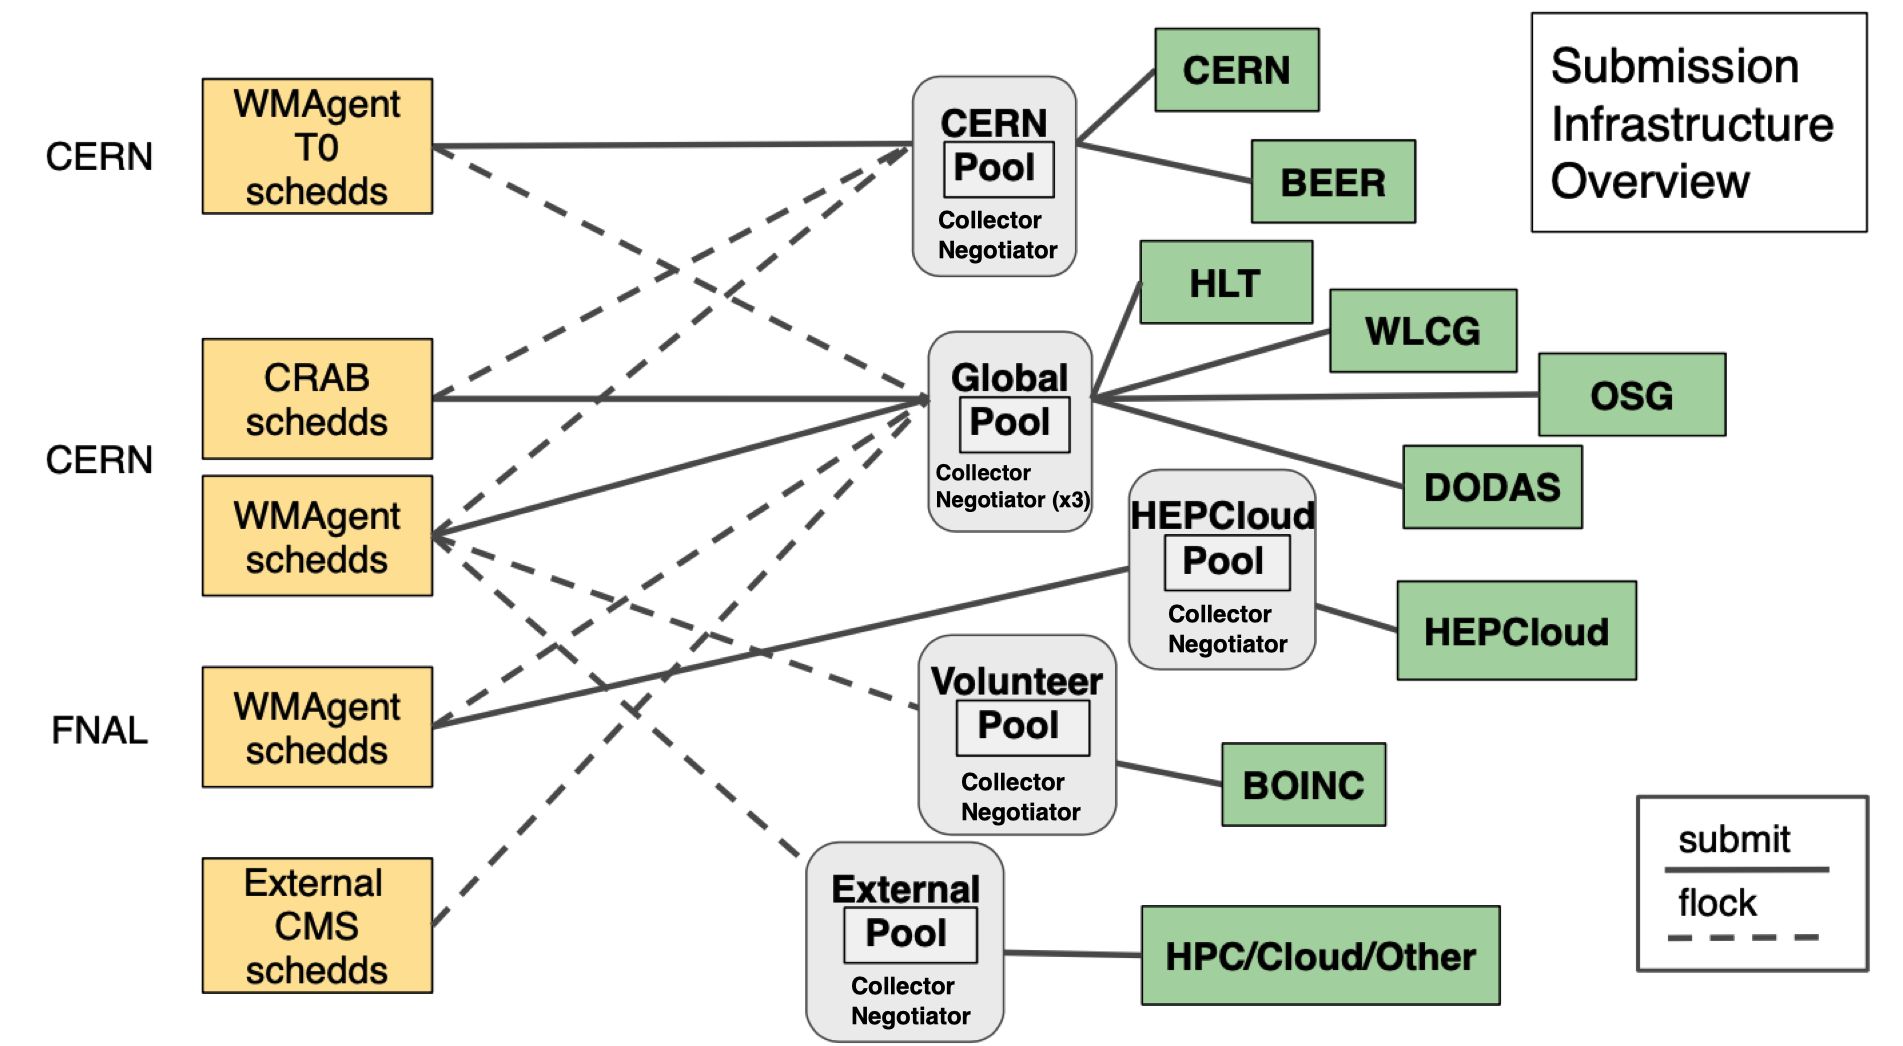
\includegraphics[width=12cm,clip]{pool_complexity_2.png}
\caption{CMS SI current configuration, including multiple federated pools of resources allocated from diverse origins (green boxes) and sets of distributed job schedulers (schedds), which can directly $submit$, or indirectly $flock$, jobs into resources supporting CMS.} 
\label{fig-SubInf}
\end{figure}

\subsection{Allocating GPU resources with GlideinWMS}
GlideinWMS supports the use of GPU resources, with the Front-End (FE) and factory components being capable of defining and submitting pilot jobs requesting heterogeneous resources~\cite{gpu_glideinwms}. As in the case for CPUs pilots, GPU requests are negotiated with the remote Compute Elements (CE) at each Grid site. The number of GPUs per pilot, along with other usual attributes (CPUs, memory, etc) can be predefined at the factory entry level, although additional attributes can be setup dynamically via the FE group description.

In the Global Pool, each GlideinWMS pilot job runs a HTCondor startd, instantiating a partitionable slot, representing a set of resources which can be fragmented and assigned to payload jobs in a dynamic way. GPUs can be added to the partitionable slot, or alternatively, by using the GlideinWMS GLIDEIN\_Resource\_Slots parameter~\cite{gpu_glideinwms}, a specialized secondary GPU-slot can be added on to the main one. 

Once allocated, GPU resources need to be properly identified and described, for example using TotalSlotGPUs, a partitionable quantity analogous to TotalSlotCPUs, but also employing extra tags such as CUDACapability, CUDARuntimeVersion, CUDAGlobalMemoryMb, etc. If the slot is not (completely) predefined from the factory and FE requests, GlideinWMS pilots can make use of the condor\_gpu\_discovery tool~\cite{gpu_discover1}~\cite{gpu_discover2}, a binary provided by HTCondor and shipped with every pilot that can set up multiple attributes to the slot description.

%The \emph{auto} is also available in case of a normal (non whole node) pilot, but it should be avoided because otherwise multiple pilots running on the same node are going to be competing for the same resources. Possibly, pilots from different VOs could be running on a node.
%Similarly, any auto-discovery strategy that might be being implemented independently at the CMSSW experiment framework level, or at any other intermediate layer (e.g.: workload management), has to be avoided in order to not incur in redundant conflicting information and configurations, which might lead to sub optimal utilization. 

\subsection{Matchmaking workloads requesting GPUs} 
HTCondor considers GPUs just as another resource to be matched to jobs~\cite{gpu_condor}. All jobs that intend to use GPUs must request this resource in their condor submit file (along with the usual requests for CPUs, memory and disk). For example:

\begin{verbatim}
request_gpus = 1
\end{verbatim}

Jobs can make use of the GPUs by employing an API such as OpenCL or CUDA. Therefore, in case a specific version of CUDA, a certain type of GPU, or any other specialized attribute is needed, corresponding requirements can be added to the condor jdl submit file. For example, if a job needs a certain version of the CUDA libraries, it should include:
\begin{verbatim}
requirements = (CUDARuntimeVersion >= 4.0) && (CUDACapability > 3.0)
\end{verbatim}

\subsection{Accessing software libraries}
Certain software libraries need to be available in order for dedicated programs to make effective use of the GPU slots. As in the general case, jobs access all required software, including CMSSW and singularity images, via CVMFS~\cite{cvmfs}. The use of CVMFS, along with the GlideinWMS tools managing the proper configuration of the pilots, ensure that all needed software is available and correctly located in the payload job runtime environment. 

Payload GPU jobs are executed in singularity containers~\cite{sing_gpu}, just as in the general case for all CMS payloads. Some jobs may be required to run in specialized singularity containers. For example, Tensorflow jobs can make use of the ready-to-use singularity containers provided by the Open Science Grid (OSG), for for both CPU and GPU jobs~\cite{tensorflow}. These containers are based on Ubuntu and distributed via CVMFS. The OSG also maintains versions of the CUDA Deep Neural Network library (cuDNN), Keras, etc. 

The CMS Connect service allows access to GPU resources in the Global Pool, providing documentation on how to request and use them (see~\cite{tensorflow_usage} for an example on how to use TensorFlow with GPU resources). In particular a SingularityImage attribute is employed to determine the predefined container suitable to the execution of the payload, for example:
\begin{verbatim}
+SingularityImage = "/cvmfs/singularity.opensciencegrid.org/open\
sciencegrid/tensorflow-gpu:latest"
\end{verbatim}

\subsection{Running multiple jobs simultaneously on a single GPU}
Allowing multiple jobs to utilize a single GPU would be in principle helpful to run workloads or jobs that do not consume the entire GPU (in terms of memory or processing). HTCondor developers are aware of this possibility, noting that NVIDIA is adding the ability to share a GPU between processes in newer hardware with hardware enforcement of memory isolation between processes~\cite{nvidia}. HTCondor developers have expressed their interest and plan to support it in the future. 
 
\subsection{Interactive use of GPU resources}
GPU resources can in principle be accessed interactively via condor\_ssh\_to\_job~\cite{ssh_to_job}. This is potentially a very interesting possibility for analysis users, helping them reduce the delay between analysis cycles. However, it's presently regarded as an expert mode of operations, which requires some manipulation of the ssh options in order to enter the singularity container, which can be configured to load the GPU libraries inherited from the host, instead of a plain starter mode.  

%However, some changes might still be needed at the pilot level, that we need to investigate (sshd available in the containers, STARTD configuration accepting SSH connections, etc). There is also one issue with condor that affect GPUs. We use the singularity --nv option to link the GPU libraries from the host into the container, which is set inside the container through some bindings and environment variables. We lose the environment with condor\_ssh\_to\_job at present, because condor grabs the environment of the starter, rather than the childs (the singularity process spawned). I created an condor issue here, describing the issue in detail? https://htcondor-wiki.cs.wisc.edu/index.cgi/tktview?tn=7636  

\subsection{Accounting for GPUs}
The concepts of resource accounting and fair-share are essential in an HTCondor pool employed by multiple users. It is thus necessary to determine the amount of resources that have been consumed by  (and should be assigned to) each user. The default resource accounting is performed on the basis of how many CPUs the user jobs are have consumed and for how long. However, when GPUs are also utilized, a redefined ``slot weight'', considering also the GPUs usage must be considered. GPU slots would otherwise be treated as an infinite resource, added with no cost along with the weighted CPU cores. The CMS SI team has planned the introduction of an exclusive HTCondor $negotiator$ to manage the matchmaking of heterogeneous resources, in order to incorporate a cost to using GPUs, which can be the basis of a fair-share based access to GPUs.

% ================

\section{GPU resources currently available in the CMS Global Pool}
\label{sec:status}
Even though, to this date, CMS has not officially requested its supporting computing centers to provide any GPU slots, a number of sites are already advertising and allowing exploitation of GPUs by CMS users opportunistically, accepting pilot jobs from the Global Pool that have been tuned to acquire these resources. Heterogeneous clusters are currently mainly available to CMS in Tier-2 sites in the USA (Nebraska, Vanderbilt, Syracuse, Purdue, Wisconsin and UCSD), while the contribution from EU sites is growing as well (e.g. KIT). 

GlideinWMS GPU pilots are only submitted to sites when jobs specify GPU resources in their requirements. Jobs requests may include several GPU characteristics in order to target any of the available resources in particular. 

In order to make their access easier for CMS users, the SI team has setup an automated system that periodically scans the Global Pool for GPU resources. Pilot jobs are automatically submitted to CMS sites allowing GPU allocation, as defined according to the factories entries. Pilots gather information about the GPU resources found in the execution nodes they are assigned to using the condor\_gpu\_discovery tool describe above. 

This information collected is then advertised via a dedicated dashboard, deployed in the CMS SI monitoring environment, accessible to CMS users interested in utilizing GPUs. Figure~\ref{fig-GPUResources} shows an example of the main element in this dashboard, a full table listing resources, their location and their main characteristics. It is essential that this dashboard information is always maintained up to date, as the list of resources is in constant and fast evolution.

\begin{figure}[h]
\centering
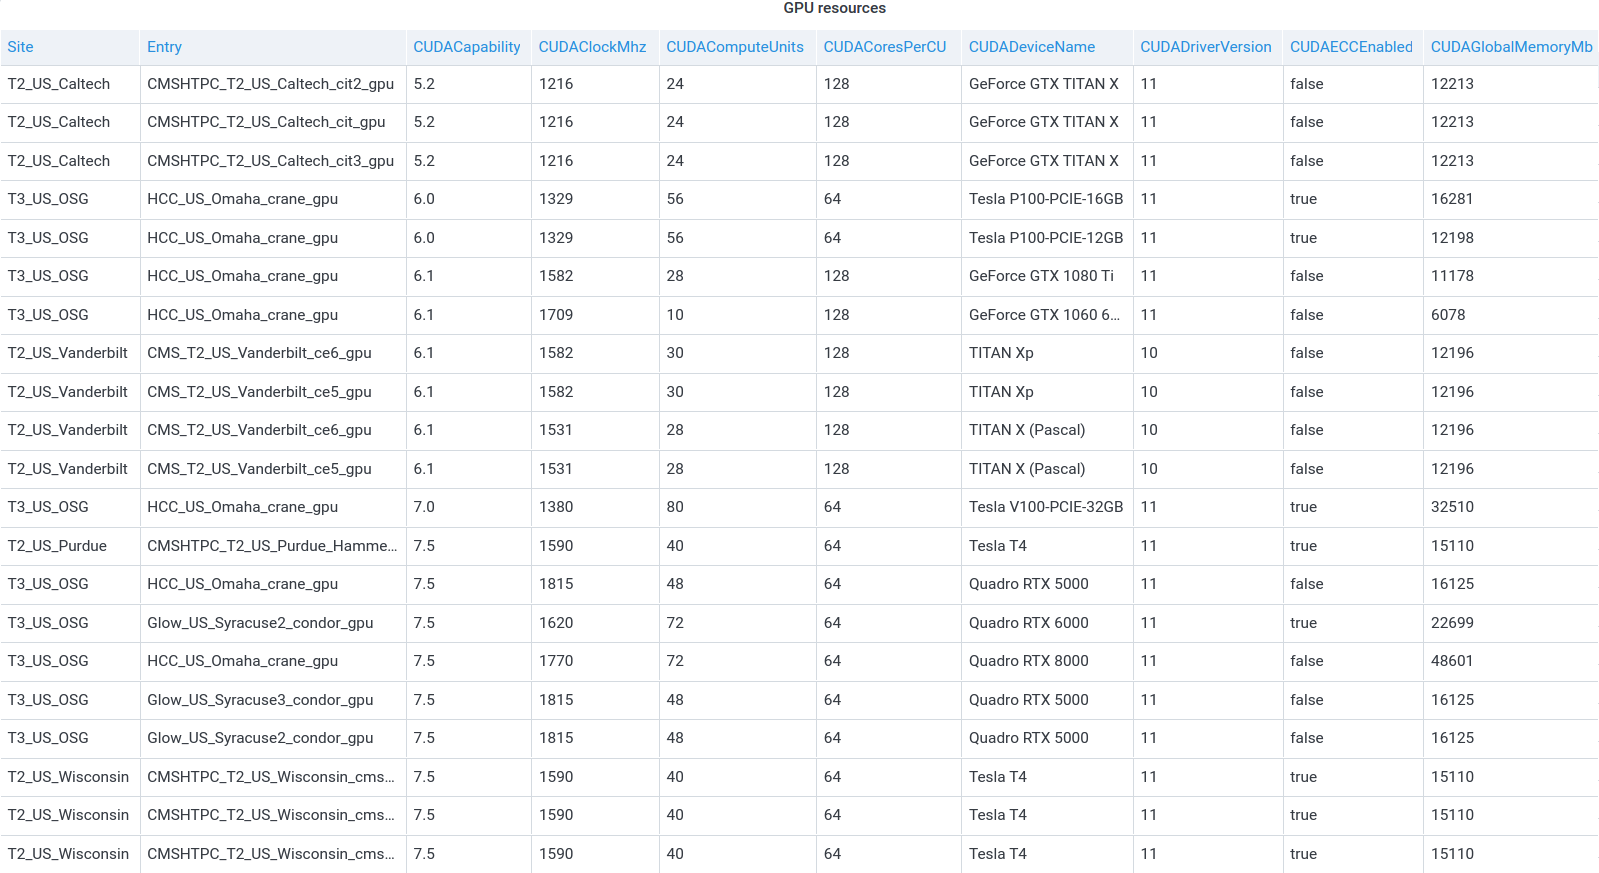
\includegraphics[width=13cm]{GPUResources_2.png}
\setlength{\belowcaptionskip}{-20pt}
\caption{CMS SI dashboard containing information about GPU slots in the Global Pool, showing a subset of the presently available resources.}
\label{fig-GPUResources}       % Give a unique label
\end{figure}

% =============

\section{Conclusions}
\label{sec:conclusions}
This paper has summarized the challenges and evolution that the CMS Submission Infrastructure is facing in order to ensure access and make effective use of heterogeneous resources by CMS. While all the basic tools directly involved in the CMS Global Pool are in principle ready (and in fact, being used at small scale already), a number of questions related to the preferred mode of operations remain unsolved. An iterative process should clarify the advantages or limitations of the diverse models described, for example in the use of exclusive or heterogeneous clusters, the submission of specialized or generic workflows with regards to the use of CPUs and GPUs, etc. 

The GlideinWMS resource provisioning system already supports the creation of pilots for GPU-like slots and the use of singularity images with specific software libraries. Matchmaking of jobs to GPUs can be done using a simple extension of the HTCondor classads machinery, supporting a description based on very specific attributes. A key element is thus having workflows and resources properly tagged. However, as noted, an excessively fine granularity in the description of GPU resources and workload requirements may be detrimental to their overall efficiency of use.

CMS users can already access a growing number of GPU resources available in the Global Pool. However, the management of resource accounting, fair-shares and quotas is still based solely on CPUs, which needs to be developed to include GPUs in the near future. 

\section*{}
\label{acknowledgements}
\begin{acknowledgement}
A. P\'erez-Calero Yzquierdo acknowledges support by Spain’s Ministry of Economy and Competitiveness grant FPA2016-80994.
\end{acknowledgement}

%------------

\begin{thebibliography}{}
%\bibitem{RefJ} Journal Author, Journal \textbf{Volume}, page numbers (year)
\bibitem{gwms} The Glidein-based Workflow Management System, \url{https://glideinwms.fnal.gov/doc.prd/index.html}
\bibitem{htcondor} HTCondor public web site, \url{https://research.cs.wisc.edu/htcondor/index.html}
\bibitem{global_pool} J. Balcas et al. ``Using the glideinWMS System as a Common Resource Provisioning Layer in CMS'', J. Phys.: Conf. Ser. \textbf{664} 062031 (2015).
\bibitem{hpc} A. P\'erez-Calero Yzquierdo et al. ``CMS Strategy for HPC resource exploitation'', EPJ Web of Conferences \textbf{245}, 09012 (2020).
\bibitem{cms_hllhc} CMS Offline and Computing Public Results, \url{https://twiki.cern.ch/twiki/bin/view/CMSPublic/CMSOfflineComputingResults}, accessed February, 2021.
\bibitem{cms_RandD} CMS Offline Software and Computing. ``Evolution of the CMS Computing Model towards Phase-2'', CMS NOTE-2021/001 (2021)
\bibitem{gpus_track} A. Bocci et al. ``Heterogeneous Reconstruction of Tracks and Primary Vertices With the CMS Pixel Tracker'', Frontiers in Big Data \textbf{3}, 49 (2020). 
\bibitem{gpus_hlt} A. Bocci. ``Heterogeneous online reconstruction at CMS'' (2019) \url{https: //indico.cern.ch/event/773049/contributions/3474336/}, accessed February, 2021.
%\bibitem{vocard} \url{https://operations-portal.egi.eu/vo/view/voname/cms}
\bibitem{multicore} A. P\'erez-Calero Yzquierdo et al. ``CMS readiness for multi-core workload scheduling'', J. Phys.: Conf. Ser. \textbf{898}, 052030 (2017).
\bibitem{wlcg} The Worldwide LHC Computing Grid \url{http://wlcg.web.cern.ch}, accessed February, 2021.
\bibitem{dodas} D. Spiga et al. ``Exploiting private and commercial clouds to generate on-demand CMS computing facilities with DODAS'', EPJ Web of Conferences. \textbf{214}. 07027 (2019). 
\bibitem{boinc} D. P. Anderson. ``BOINC: A Platform for Volunteer Computing'', J Grid Computing (2019).
%\bibitem{lhcathome} LHC at Home, \url{https://lhcathome.cern.ch/}, accessed February, 2021.
\bibitem{hlt} D. Da Silva Gomes et al. ``Experience with dynamic resource provisioning of the CMS online cluster using a cloud overlay'', EPJ Web of Conferences. \textbf{214}. 07017 (2019).
\bibitem{cineca} Consorzio Interuniversitario del Nordest Italiano Per il Calcolo Automatico (CINECA) \url{https://www.cineca.it}, accessed February, 2021.
\bibitem{kit} M. Schnepf et al. "Dynamic Integration and Management of Opportunistic Re- sources for HEP", EPJ Web of Conferences \textbf{214}, 08009 (2019).
%\bibitem{beer} D. Smith et al. ``Sharing server nodes for storage and computer'', EPJ Web of Conferences. \textbf{214}. 08025 (2019).
%\bibitem{azure} D. Giordano et al. ``CERN-IT evaluation of Microsoft Azure cloud IaaS, '', \url{https://zenodo.org/record/48495#.X9I7JC8rx24}, accessed February, 2021.
\bibitem{hepcloud} S. Timm et al. ``Virtual machine provisioning, code management, and data movement design for the Fermilab HEPCloud Facility'', J. Phys.: Conf. Ser. \textbf{898} 052041 (2017).
\bibitem{nersc} National Energy Research Scientific Computing Center (NERSC) \url{https://www.nersc.gov}, accessed February, 2021.
%\bibitem{wmagent} E Fajardo et al. ``A new era for central processing and production in CMS'', J. Phys.: Conf. Ser. \textbf{396} 042018 (2012).
\bibitem{gpu_glideinwms} ``GlideinWMS Factory, Custom HTCondor Variables'', \url{https://glideinwms.fnal.gov/doc.prd/factory/custom_vars.html}, accessed February, 2021.
\bibitem{gpu_discover1} ``HTCondor Reference Manual: condor\_gpu\_discovery'', \url{https://htcondor.readthedocs.io/en/latest/man-pages/condor_gpu_discovery.html}, accessed February, 2021.
\bibitem{gpu_discover2}``How to Manage GPUs'', \url{https://htcondor-wiki.cs.wisc.edu/index.cgi/wiki?p=HowToManageGpus}, accessed February, 2021.
\bibitem{gpu_condor} ``Jobs That Use GPUs'', \url{http://chtc.cs.wisc.edu/gpu-jobs.shtml}, accessed February, 2021.
\bibitem{cvmfs} ``About CernVM-FS'', \url{https://cernvm.cern.ch/fs/}, accessed February, 2021.
\bibitem{sing_gpu} ``Singularity GPU Support (NVIDIA CUDA \& AMD ROCm)'', \url{https://sylabs.io/guides/3.5/user-guide/gpu.html}, accessed February, 2021.
\bibitem{tensorflow} ``OSGVO's TensorFlow base image definitions, with GPU components, for Docker and Singularity'', \url{https://github.com/opensciencegrid/osgvo-tensorflow-gpu}, accessed February, 2021.
\bibitem{tensorflow_usage} ``CMS Connect Handbook. Using TensorFlow'', \url{http://docs.uscms.org/Using+TensorFlow}, accessed February, 2021.
\bibitem{nvidia} ``Multi-Process Service'', \url{https://docs.nvidia.com/deploy/mps/index.html}, accessed February, 2021.
\bibitem{ssh_to_job} ``CMS Connect Handbook. Using GPU resources via SSH'' \url{https://ci-connect.atlassian.net/wiki/spaces/CMS/pages/804519939/Using+GPU+resources+via+SSH}, accessed February, 2021.

%------------
%\bibitem{RefJ} \url{https://indico.cern.ch/event/689511/contributions/2882023/attachments/1599859/2536058/WLCG_GPUS_OSG_CMS_v0_1.pdf}
%\bibitem{RefJ} \url{https://github.com/opensciencegrid/osgvo-el7}
%\bibitem{RefJ} \url{http://docs.uscms.org/Using+TensorFlow}
%\bibitem{RefJ} \url{https://htcondor-wiki.cs.wisc.edu/index.cgi/tktview?tn=7018}
%\bibitem{RefJ} \url{https://htcondor-wiki.cs.wisc.edu/index.cgi/tktview?tn=6825}
%\bibitem{RefJ} \url{https://htcondor-wiki.cs.wisc.edu/index.cgi/tktview?tn=6934}
%------------
\end{thebibliography}

\end{document}
%--------------